\chapter{Georeferencing}
\section{Objective of the exercise}
Hard copy maps are one of the important sources of inputs in GIS. Generally, these maps are scanned so that they can be visualized/analyzed in GIS. However, scanning the maps is not enough to overlay over other features. It is necessary to georeference these scanned maps. In this exercise, you will learn to georeference a map.

\section{Data}
The data for this exercise is in the \emph{georef} folder. You will use the following data and information.
\begin{enumerate}
\item{Tamakoshi.tif | It is a scanned map which is to be georeferenced}
\item{Coordinates | This file contains the coordinates that you will use to georeference the map.}
\item{NEPAL\textunderscore MUTM\textunderscore CM\textunderscore EVEREST\textunderscore 1830.prj | Projection system of the map}
\end{enumerate}

\section{Steps}
\subsection{Open ArcMap and Set the Coordinate System}
\begin{enumerate}
\item{Go to View | Data Frame Properties | Coordinate System}
\item{Import the NEPAL\textunderscore MUTM\textunderscore CM\textunderscore EVEREST\textunderscore 1830.prj from \emph{Georef} folder as shown in fig \ref{coordinate_system} }
\begin{figure}[h]
\label{coordinate_system}
\centering
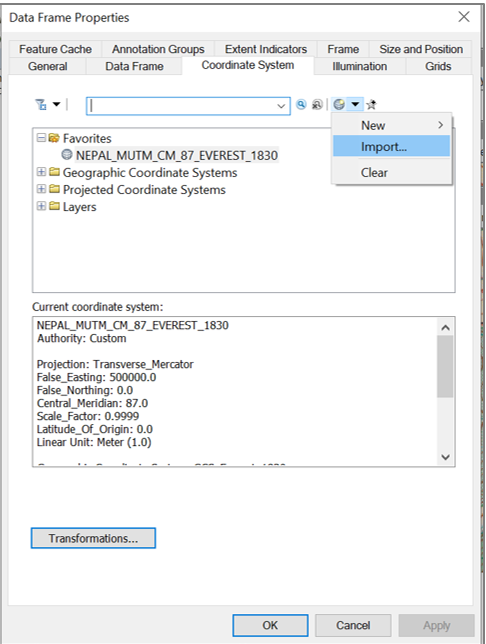
\includegraphics[scale=0.5]{images/coordinate_system}
\caption{Import Coordinate System}
\end{figure}
\end{enumerate}

\subsection{Add the scanned map} 
\begin{enumerate}
\item{Add the scanned map into ArcMap | Tamakoshi.tif}
\item{Check the coordinates (right-bottom) on Arcmap as you move the mouse over the image.}
\end{enumerate}

\subsection{Add Georeferencing toolbar}
\begin{enumerate}
\item{Select Customize | Toolbars | Georeferencing to add the Georeferencing toolbar as shown in figure}
\item{Hover over each tool icon in the Georeferencing toolbar and note their name}
item{Select \emph{Georeferencing}  and uncheck Auto Adjust}
\end{enumerate}

\subsection{Georeferencing}
\begin{enumerate}
\item{Select \emph{Add Control Points}, zoom to the intersection of grid lines towards each corner of the image. We know the coordinates of these point of map}
\item{First click on left mouse key, then click on right mouse click and select Input X and Y.} 
\item{Put the coordinates as per the excel file: Georeferencing Coordinates}
\item{Once done, click \emph{Georeferencing | Update Georeferencing}}
\item{Now you can check the coordinates. Now, the coordinates are real world coordinates.}
\item{Add Rivers from \emph{nepal\textunderscore data} folder. The rivers (vector layer) must overlay over the map.}
\end{enumerate}

\subsection{Georefencing Exercise}
\begin{enumerate}
\item{Use the raster map, coordinate data and coordinate system file in \emph{exercise\textunderscore georef} folder to georeference the \emph{lamabagar.tif} map.}
\item{Once done, check it by overlaying with the river vector layer from \emph{nepal\textunderscore data} folder.}
\end{enumerate}

